\documentclass[12pt,a4paper]{article}
\usepackage{lmodern}
\usepackage{amssymb,amsmath}
\usepackage{ifxetex,ifluatex}
\usepackage{fixltx2e} % provides \textsubscript
\ifnum 0\ifxetex 1\fi\ifluatex 1\fi=0 % if pdftex
  \usepackage[T1]{fontenc}
  \usepackage[utf8]{inputenc}
\else % if luatex or xelatex
  \ifxetex
    \usepackage{mathspec}
  \else
    \usepackage{fontspec}
  \fi
  \defaultfontfeatures{Ligatures=TeX,Scale=MatchLowercase}
\fi
% use upquote if available, for straight quotes in verbatim environments
\IfFileExists{upquote.sty}{\usepackage{upquote}}{}
% use microtype if available
\IfFileExists{microtype.sty}{%
\usepackage{microtype}
\UseMicrotypeSet[protrusion]{basicmath} % disable protrusion for tt fonts
}{}
\usepackage[margin=2cm]{geometry}
\usepackage{hyperref}
\PassOptionsToPackage{usenames,dvipsnames}{color} % color is loaded by hyperref
\hypersetup{unicode=true,
            pdftitle={SQUEAC Attack},
            pdfauthor={Mark Myatt},
            colorlinks=true,
            linkcolor=blue,
            citecolor=blue,
            urlcolor=blue,
            breaklinks=true}
\urlstyle{same}  % don't use monospace font for urls
\usepackage{natbib}
\bibliographystyle{plainnat}
\usepackage{color}
\usepackage{fancyvrb}
\newcommand{\VerbBar}{|}
\newcommand{\VERB}{\Verb[commandchars=\\\{\}]}
\DefineVerbatimEnvironment{Highlighting}{Verbatim}{commandchars=\\\{\}}
% Add ',fontsize=\small' for more characters per line
\usepackage{framed}
\definecolor{shadecolor}{RGB}{248,248,248}
\newenvironment{Shaded}{\begin{snugshade}}{\end{snugshade}}
\newcommand{\KeywordTok}[1]{\textcolor[rgb]{0.13,0.29,0.53}{\textbf{#1}}}
\newcommand{\DataTypeTok}[1]{\textcolor[rgb]{0.13,0.29,0.53}{#1}}
\newcommand{\DecValTok}[1]{\textcolor[rgb]{0.00,0.00,0.81}{#1}}
\newcommand{\BaseNTok}[1]{\textcolor[rgb]{0.00,0.00,0.81}{#1}}
\newcommand{\FloatTok}[1]{\textcolor[rgb]{0.00,0.00,0.81}{#1}}
\newcommand{\ConstantTok}[1]{\textcolor[rgb]{0.00,0.00,0.00}{#1}}
\newcommand{\CharTok}[1]{\textcolor[rgb]{0.31,0.60,0.02}{#1}}
\newcommand{\SpecialCharTok}[1]{\textcolor[rgb]{0.00,0.00,0.00}{#1}}
\newcommand{\StringTok}[1]{\textcolor[rgb]{0.31,0.60,0.02}{#1}}
\newcommand{\VerbatimStringTok}[1]{\textcolor[rgb]{0.31,0.60,0.02}{#1}}
\newcommand{\SpecialStringTok}[1]{\textcolor[rgb]{0.31,0.60,0.02}{#1}}
\newcommand{\ImportTok}[1]{#1}
\newcommand{\CommentTok}[1]{\textcolor[rgb]{0.56,0.35,0.01}{\textit{#1}}}
\newcommand{\DocumentationTok}[1]{\textcolor[rgb]{0.56,0.35,0.01}{\textbf{\textit{#1}}}}
\newcommand{\AnnotationTok}[1]{\textcolor[rgb]{0.56,0.35,0.01}{\textbf{\textit{#1}}}}
\newcommand{\CommentVarTok}[1]{\textcolor[rgb]{0.56,0.35,0.01}{\textbf{\textit{#1}}}}
\newcommand{\OtherTok}[1]{\textcolor[rgb]{0.56,0.35,0.01}{#1}}
\newcommand{\FunctionTok}[1]{\textcolor[rgb]{0.00,0.00,0.00}{#1}}
\newcommand{\VariableTok}[1]{\textcolor[rgb]{0.00,0.00,0.00}{#1}}
\newcommand{\ControlFlowTok}[1]{\textcolor[rgb]{0.13,0.29,0.53}{\textbf{#1}}}
\newcommand{\OperatorTok}[1]{\textcolor[rgb]{0.81,0.36,0.00}{\textbf{#1}}}
\newcommand{\BuiltInTok}[1]{#1}
\newcommand{\ExtensionTok}[1]{#1}
\newcommand{\PreprocessorTok}[1]{\textcolor[rgb]{0.56,0.35,0.01}{\textit{#1}}}
\newcommand{\AttributeTok}[1]{\textcolor[rgb]{0.77,0.63,0.00}{#1}}
\newcommand{\RegionMarkerTok}[1]{#1}
\newcommand{\InformationTok}[1]{\textcolor[rgb]{0.56,0.35,0.01}{\textbf{\textit{#1}}}}
\newcommand{\WarningTok}[1]{\textcolor[rgb]{0.56,0.35,0.01}{\textbf{\textit{#1}}}}
\newcommand{\AlertTok}[1]{\textcolor[rgb]{0.94,0.16,0.16}{#1}}
\newcommand{\ErrorTok}[1]{\textcolor[rgb]{0.64,0.00,0.00}{\textbf{#1}}}
\newcommand{\NormalTok}[1]{#1}
\usepackage{longtable,booktabs}
\usepackage{graphicx,grffile}
\makeatletter
\def\maxwidth{\ifdim\Gin@nat@width>\linewidth\linewidth\else\Gin@nat@width\fi}
\def\maxheight{\ifdim\Gin@nat@height>\textheight\textheight\else\Gin@nat@height\fi}
\makeatother
% Scale images if necessary, so that they will not overflow the page
% margins by default, and it is still possible to overwrite the defaults
% using explicit options in \includegraphics[width, height, ...]{}
\setkeys{Gin}{width=\maxwidth,height=\maxheight,keepaspectratio}
\IfFileExists{parskip.sty}{%
\usepackage{parskip}
}{% else
\setlength{\parindent}{0pt}
\setlength{\parskip}{6pt plus 2pt minus 1pt}
}
\setlength{\emergencystretch}{3em}  % prevent overfull lines
\providecommand{\tightlist}{%
  \setlength{\itemsep}{0pt}\setlength{\parskip}{0pt}}
\setcounter{secnumdepth}{5}
% Redefines (sub)paragraphs to behave more like sections
\ifx\paragraph\undefined\else
\let\oldparagraph\paragraph
\renewcommand{\paragraph}[1]{\oldparagraph{#1}\mbox{}}
\fi
\ifx\subparagraph\undefined\else
\let\oldsubparagraph\subparagraph
\renewcommand{\subparagraph}[1]{\oldsubparagraph{#1}\mbox{}}
\fi

%%% Use protect on footnotes to avoid problems with footnotes in titles
\let\rmarkdownfootnote\footnote%
\def\footnote{\protect\rmarkdownfootnote}

%%% Change title format to be more compact
\usepackage{titling}

% Create subtitle command for use in maketitle
\newcommand{\subtitle}[1]{
  \posttitle{
    \begin{center}\large#1\end{center}
    }
}

\setlength{\droptitle}{-2em}

  \title{SQUEAC Attack}
    \pretitle{\vspace{\droptitle}\centering\huge}
  \posttitle{\par}
    \author{Mark Myatt}
    \preauthor{\centering\large\emph}
  \postauthor{\par}
      \predate{\centering\large\emph}
  \postdate{\par}
    \date{32 July 2018}

\usepackage{float} 
\usepackage{setspace}
\usepackage[utf8]{inputenc}
\onehalfspacing
\usepackage{booktabs}
\usepackage{longtable}
\usepackage{array}
\usepackage{multirow}
\usepackage[table]{xcolor}
\usepackage{wrapfig}
\usepackage{float}
\usepackage{colortbl}
\usepackage{pdflscape}
\usepackage{tabu}
\usepackage{threeparttable}
\usepackage{threeparttablex}
\usepackage[normalem]{ulem}
\usepackage{makecell}

\begin{document}
\maketitle

{
\hypersetup{linkcolor=black}
\setcounter{tocdepth}{2}
\tableofcontents
}
\newpage

\hypertarget{k}{%
\section{Calculate `k' for single coverage estimate}\label{k}}

Correction factor \texttt{k} is the ratio of the mean length of an
untreated episode to the mean length of a CMAM treatment episode.

~

\[ k ~ = ~ \frac{\text{Mean length of an untreated episode}}{\text{Mean length of a successful treatment episode}} \]

~

Mean length of an untreated episode for SAM or MAM can be assumed as 7.5
months based on \citet{Garenne:2009fq}. Mean length of a successful
treatment episode can be estimated from routine programming monitoring
data by calculating the median length of stay.

This can be implemented in R as follows:

~

\begin{Shaded}
\begin{Highlighting}[]
\NormalTok{medianLOS <-}\StringTok{ }\KeywordTok{median}\NormalTok{(work}\OperatorTok{$}\NormalTok{medianLOS, }\DataTypeTok{na.rm =} \OtherTok{TRUE}\NormalTok{)}

\NormalTok{k <-}\StringTok{ }\NormalTok{((}\FloatTok{7.5} \OperatorTok{*}\StringTok{ }\FloatTok{30.44}\NormalTok{) }\OperatorTok{/}\StringTok{ }\DecValTok{7}\NormalTok{) }\OperatorTok{/}\StringTok{ }\NormalTok{work}\OperatorTok{$}\NormalTok{medianLOS}
\end{Highlighting}
\end{Shaded}

~

The \textbf{median of the median length of stay} of the surveys in the
dataset is 7.

The \texttt{k} values for each of the surveys in the dataset
are\footnote{\texttt{NA} values are for surveys that don't report a
  median length of stay.}:

~

\begin{verbatim}
##   [1]        NA        NA        NA        NA        NA        NA        NA
##   [8]        NA        NA        NA        NA        NA        NA        NA
##  [15]        NA        NA        NA        NA  4.076786        NA        NA
##  [22]        NA        NA  4.076786  4.659184  6.522857        NA  4.076786
##  [29]  8.153571  3.623810  4.076786        NA  3.623810        NA  5.435714
##  [36]  5.435714        NA        NA  3.623810        NA  3.623810        NA
##  [43]        NA        NA        NA        NA  3.261429  3.261429  4.076786
##  [50]  3.623810        NA  4.076786  4.076786  2.964935        NA  2.717857
##  [57]  8.153571  4.076786  4.076786  3.623810        NA        NA  8.153571
##  [64]        NA        NA  5.435714  5.435714  6.522857  8.153571  6.522857
##  [71]        NA  5.435714  6.522857  5.435714  3.623810  6.522857  8.153571
##  [78]  4.659184        NA  6.522857        NA  6.522857        NA  5.435714
##  [85]  3.623810  4.659184  4.076786        NA  5.435714        NA  5.435714
##  [92]  2.964935  4.076786 10.871429  2.717857        NA        NA        NA
##  [99]        NA  3.261429  4.076786  4.659184  4.076786  4.659184  5.435714
## [106]        NA        NA        NA        NA        NA        NA  4.659184
## [113]        NA  3.623810        NA        NA  3.623810        NA        NA
## [120]  4.659184  2.717857  4.659184        NA  4.076786  4.659184  3.623810
## [127]  6.522857  5.435714  8.153571  5.435714  5.435714  5.435714  4.659184
## [134]  6.522857  6.522857  6.522857  5.435714        NA  6.522857  4.659184
## [141]  4.659184        NA  5.435714        NA  5.435714  5.435714        NA
## [148]  5.435714  4.076786  5.435714  4.076786  4.076786        NA  4.659184
## [155]  8.153571  8.153571        NA  8.153571        NA  5.435714  4.659184
## [162]  6.522857  8.153571  8.153571  8.153571        NA  8.153571  8.153571
## [169]        NA        NA  5.435714        NA        NA        NA  8.153571
## [176]  6.522857  6.522857  3.261429  6.522857  5.435714  8.153571  4.659184
## [183]  5.435714  4.076786  4.659184  4.076786        NA  4.659184        NA
## [190]  6.522857 10.871429  6.522857  5.435714  4.659184  8.153571  5.435714
## [197]  6.522857  6.522857  5.435714  5.435714  3.623810        NA  3.623810
## [204]  5.435714  6.522857  4.659184  3.261429  2.964935  3.261429  3.261429
## [211]  3.623810  5.435714  3.623810  5.435714  4.076786  5.435714  4.076786
## [218]  5.435714        NA        NA  4.076786  4.659184  4.659184  3.623810
## [225]  4.659184        NA        NA        NA  3.623810  5.435714        NA
## [232]  4.659184  5.435714        NA  2.717857        NA  6.522857  6.522857
## [239]  6.522857  6.522857        NA  4.076786        NA  8.153571  3.623810
## [246]  5.435714        NA  2.508791  2.174286        NA  4.076786  2.964935
## [253]  4.659184  3.623810        NA        NA  5.435714  2.508791  5.435714
## [260]  4.076786        NA        NA  3.623810  4.659184        NA  6.522857
## [267]  5.435714  3.261429  4.659184  5.435714  5.435714  3.623810        NA
## [274]  4.659184  4.076786        NA  4.659184  5.435714  5.435714  6.522857
## [281]  2.964935  4.659184  5.435714        NA        NA
\end{verbatim}

\newpage

\hypertarget{r.out}{%
\section{Calculate r.out (recovering cases NOT in the
program)}\label{r.out}}

Using the calculated \texttt{k} values in previous section, number of
recovering cases NOT in the program is calculated using the following
formula:

~

\[\begin{aligned}
R_{out} & ~ \approx ~ \frac{1}{k} ~ \times ~ \left ( ~ R_{in} ~ \times ~ \frac{C_{in} ~ + ~ C_{out} ~ + ~ 1}{C_{in} ~ + ~ 1} ~ - ~ R_{in} ~ \right ) \\
\\
where: & \\
\\
k & ~ = ~ \text{correction factor} \\
C_{in} & ~ = ~ \text{current SAM cases in the program} \\
C_{out} & ~ = ~ \text{current SAM cases not in the program} \\ 
R_{in} & ~ = ~ \text{recovering SAM cases in the program}
\end{aligned}\]

~

This can be implemented in R as follows:

~

\begin{Shaded}
\begin{Highlighting}[]
\NormalTok{r.out <-}\StringTok{ }\KeywordTok{floor}\NormalTok{((}\DecValTok{1} \OperatorTok{/}\StringTok{ }\NormalTok{k) }\OperatorTok{*}\StringTok{ }
\StringTok{                 }\NormalTok{(work}\OperatorTok{$}\NormalTok{r.in }\OperatorTok{*}\StringTok{ }\NormalTok{((work}\OperatorTok{$}\NormalTok{c.in }\OperatorTok{+}\StringTok{ }\NormalTok{work}\OperatorTok{$}\NormalTok{c.out }\OperatorTok{+}\StringTok{ }\DecValTok{1}\NormalTok{) }\OperatorTok{/}\StringTok{ }
\StringTok{                                 }\NormalTok{(work}\OperatorTok{$}\NormalTok{c.in }\OperatorTok{+}\StringTok{ }\DecValTok{1}\NormalTok{)) }\OperatorTok{-}\StringTok{ }\NormalTok{work}\OperatorTok{$}\NormalTok{r.in))}
\end{Highlighting}
\end{Shaded}

~

The resulting vector of \texttt{r.out} values are:

~

\begin{verbatim}
##   [1]  NA  NA  NA  NA  NA  NA  NA  NA  NA  NA  NA  NA  NA  NA  NA  NA  NA
##  [18]  NA   4  NA  NA  NA  NA  10   1   7  NA  NA   2  NA   5  NA  NA  NA
##  [35]  NA  NA  NA  NA  NA  NA   2  NA  NA  NA  NA  NA   3  NA   5   2  NA
##  [52]  NA   3  22  NA  NA   2  21   4   0  NA  NA  NA  NA  NA  NA  10   0
##  [69]  NA  NA  NA   9   6   6   0  21  NA   4  NA  NA  NA   1  NA   2   9
##  [86]  NA  NA  NA   0  NA   3  NA   4  NA  NA  NA  NA  NA  NA  NA  NA   3
## [103]  15   0   1  NA  NA  NA  NA  NA  NA   3  NA  13  NA  NA   3  NA  NA
## [120]   1   5   2  NA  NA  NA  NA   6  14  NA   4  NA  NA  NA   8   4  NA
## [137]   2  NA  16  NA  11  NA  NA  NA   8   8  NA   1  NA  30  21  21  NA
## [154]   2  NA   5  NA   5  NA  NA  NA  NA   9  NA   8  NA  NA  NA  NA  NA
## [171]   7  NA  NA  NA   2   2   1  15   6  NA   0  NA  NA   3  10   5  NA
## [188]  11  NA   2   6   2   1   2  10  14   1   8  NA  NA  NA  NA  NA   7
## [205]   1   5 179  12   3   4   6   6   0   4   2   5   6   1  NA  NA   0
## [222]  NA  NA   3  12  NA  NA  NA   2  21  NA  NA   0  NA  11  NA   0  NA
## [239]  NA  NA  NA   0  NA  NA   1  NA  NA  12  16  NA  NA   7   0  NA  NA
## [256]  NA   0   7  NA  NA  NA  NA  16  11  NA   5  NA   5   2   0   1   6
## [273]  NA  11  10  NA   0  10   0   0   2   5   4  NA  NA
\end{verbatim}

\newpage

\hypertarget{calculate-prior-modes-priormode-from-prioralpha-and-priorbeta-with-their-standard-errors-priormodese}{%
\section{Calculate Prior modes (priorMode) from priorAlpha and priorBeta
with their standard errors
(priorModeSE)}\label{calculate-prior-modes-priormode-from-prioralpha-and-priorbeta-with-their-standard-errors-priormodese}}

The Prior mode can be calculated from Prior \(\alpha\) and Prior
\(\beta\) as shown in the following formula.

~

\[ mode_{Prior} ~ = ~ \frac{\alpha_{Prior} - 1}{\alpha_{Prior} ~ + ~ \beta_{Prior} ~ - ~ 2} \]

~

This can be implemented in R as follows:

~

\begin{Shaded}
\begin{Highlighting}[]
\NormalTok{priorN <-}\StringTok{ }\NormalTok{work}\OperatorTok{$}\NormalTok{priorAlpha }\OperatorTok{-}\StringTok{ }\DecValTok{1}

\NormalTok{priorD <-}\StringTok{ }\NormalTok{work}\OperatorTok{$}\NormalTok{priorAlpha }\OperatorTok{+}\StringTok{ }\NormalTok{work}\OperatorTok{$}\NormalTok{priorBeta }\OperatorTok{-}\StringTok{ }\DecValTok{2}

\NormalTok{priorMode <-}\StringTok{ }\NormalTok{priorN }\OperatorTok{/}\StringTok{ }\NormalTok{priorD}
\end{Highlighting}
\end{Shaded}

~

which results in:

~

\rowcolors{2}{gray!6}{white}\begin{table}[H]

\caption{\label{tab:priortable}Prior numerator, Prior denominator and Prior mode (first 20 records)}
\centering
\begin{tabular}[t]{rrr}
\hiderowcolors
\toprule
\textbf{$Prior_{numerator}$} & \textbf{$Prior_{denominator}$} & \textbf{$Prior_{mode}$}\\
\midrule
\showrowcolors
13.50 & 28.40 & 0.48\\
19.70 & 39.00 & 0.51\\
11.00 & 21.40 & 0.51\\
18.40 & 33.60 & 0.55\\
7.20 & 26.10 & 0.28\\
\addlinespace
9.50 & 24.10 & 0.39\\
8.70 & 20.60 & 0.42\\
17.20 & 34.40 & 0.50\\
9.10 & 19.00 & 0.48\\
18.50 & 33.50 & 0.55\\
\addlinespace
23.50 & 43.00 & 0.55\\
24.90 & 53.10 & 0.47\\
19.00 & 38.80 & 0.49\\
14.20 & 34.00 & 0.42\\
7.70 & 17.50 & 0.44\\
\addlinespace
32.10 & 64.50 & 0.50\\
19.70 & 39.10 & 0.50\\
21.40 & 36.70 & 0.58\\
19.80 & 34.70 & 0.57\\
10.21 & 30.03 & 0.34\\
\bottomrule
\end{tabular}
\end{table}\rowcolors{2}{white}{white}

\newpage

\hypertarget{calculate-appropriate-likelihood-numerators-liken-denominators-liked}{%
\section{Calculate appropriate likelihood numerators (likeN)
denominators
(likeD)}\label{calculate-appropriate-likelihood-numerators-liken-denominators-liked}}

The likelihood mode can be calculated depending on the coverage
estimator to assess: \emph{point coverage} or \emph{period coverage}.

~

\[\begin{aligned}
\text{Point coverage} ~ & = ~ \frac{C_{in}}{C_{in} + C_{out}} \\
\\
\text{Period coverage} ~ & = ~ \frac{C_{in} ~ + ~ R_{in}}{C_{in} ~ + ~ C_{out} ~ + ~ R_{in} ~ + ~ R_{out}}\\
\\
where: & \\
\\
C_{in} & ~ = ~ \text{current SAM cases in the program} \\
C_{out} & ~ = ~ \text{current SAM cases not in the program} \\ 
R_{in} & ~ = ~ \text{recovering SAM cases in the program} \\
R_{out} & ~ = ~ \text{recovering SAM cases not in the program}
\end{aligned}\]

~

This can be implemented in R as follows:

~

\begin{Shaded}
\begin{Highlighting}[]
\NormalTok{likeN <-}\StringTok{ }\KeywordTok{ifelse}\NormalTok{(work}\OperatorTok{$}\NormalTok{coverType }\OperatorTok{==}\StringTok{ "point"}\NormalTok{, work}\OperatorTok{$}\NormalTok{c.in, work}\OperatorTok{$}\NormalTok{c.in }\OperatorTok{+}\StringTok{ }\NormalTok{work}\OperatorTok{$}\NormalTok{r.in)}

\NormalTok{likeD <-}\StringTok{ }\KeywordTok{ifelse}\NormalTok{(work}\OperatorTok{$}\NormalTok{coverType }\OperatorTok{==}\StringTok{ "point"}\NormalTok{, work}\OperatorTok{$}\NormalTok{c.in }\OperatorTok{+}\StringTok{ }\NormalTok{work}\OperatorTok{$}\NormalTok{c.out, }
           \KeywordTok{ifelse}\NormalTok{(work}\OperatorTok{$}\NormalTok{coverType }\OperatorTok{==}\StringTok{ "period"}\NormalTok{, }
\NormalTok{                  work}\OperatorTok{$}\NormalTok{c.in }\OperatorTok{+}\StringTok{ }\NormalTok{work}\OperatorTok{$}\NormalTok{r.in }\OperatorTok{+}\StringTok{ }\NormalTok{work}\OperatorTok{$}\NormalTok{c.out, }
\NormalTok{                  work}\OperatorTok{$}\NormalTok{c.in }\OperatorTok{+}\StringTok{ }\NormalTok{work}\OperatorTok{$}\NormalTok{r.in }\OperatorTok{+}\StringTok{ }\NormalTok{work}\OperatorTok{$}\NormalTok{c.out }\OperatorTok{+}\StringTok{ }\NormalTok{r.out))}

\NormalTok{likeMode <-}\StringTok{ }\NormalTok{likeN }\OperatorTok{/}\StringTok{ }\NormalTok{likeD}
\end{Highlighting}
\end{Shaded}

~

which results in:

\rowcolors{2}{gray!6}{white}\begin{table}[H]

\caption{\label{tab:liketable}Likelihood numerator, likelihood denominator and likelihood mode}
\centering
\begin{tabular}[t]{rrr}
\hiderowcolors
\toprule
\textbf{$Likelihood_{numerator}$} & \textbf{$Likelihood_{denominator}$} & \textbf{$Likelihood_{mode}$}\\
\midrule
\showrowcolors
3 & 23 & 0.13\\
2 & 5 & 0.40\\
20 & 37 & 0.54\\
2 & 3 & 0.67\\
8 & 28 & 0.29\\
\addlinespace
8 & 13 & 0.62\\
18 & 37 & 0.49\\
4 & 11 & 0.36\\
2 & 4 & 0.50\\
5 & 6 & 0.83\\
\addlinespace
25 & 40 & 0.62\\
NA & NA & NA\\
32 & 64 & 0.50\\
25 & 88 & 0.28\\
20 & 100 & 0.20\\
\addlinespace
92 & 121 & 0.76\\
17 & 25 & 0.68\\
4 & 8 & 0.50\\
38 & 59 & 0.64\\
4 & 32 & 0.12\\
\bottomrule
\end{tabular}
\end{table}\rowcolors{2}{white}{white}

\newpage

\hypertarget{make-summary-data.frame}{%
\section{Make summary data.frame}\label{make-summary-data.frame}}

\begin{Shaded}
\begin{Highlighting}[]
\NormalTok{results <-}\StringTok{ }\KeywordTok{data.frame}\NormalTok{(priorN, priorD, priorMode, likeN, likeD, likeMode)}

\NormalTok{results <-}\StringTok{ }\NormalTok{results[}\OperatorTok{!}\KeywordTok{is.na}\NormalTok{(results}\OperatorTok{$}\NormalTok{priorMode) }\OperatorTok{&}\StringTok{ }\OperatorTok{!}\KeywordTok{is.na}\NormalTok{(results}\OperatorTok{$}\NormalTok{likeMode), ]}
\end{Highlighting}
\end{Shaded}

The resulting data.frame is:

\rowcolors{2}{gray!6}{white}\begin{table}[H]

\caption{\label{tab:resultsDF}Summary data.frame (first 30 records)}
\centering
\resizebox{\linewidth}{!}{
\begin{tabular}[t]{rrrrrr}
\hiderowcolors
\toprule
\textbf{$Prior_{numerator}$} & \textbf{$Prior_{denominator}$} & \textbf{$Prior_{mode}$} & \textbf{$Likelihood_{numerator}$} & \textbf{$Likelihood_{denominator}$} & \textbf{$Likelihood_{mode}$}\\
\midrule
\showrowcolors
13.50 & 28.40 & 0.4753521 & 3 & 23 & 0.1304348\\
19.70 & 39.00 & 0.5051282 & 2 & 5 & 0.4000000\\
11.00 & 21.40 & 0.5140187 & 20 & 37 & 0.5405405\\
18.40 & 33.60 & 0.5476190 & 2 & 3 & 0.6666667\\
7.20 & 26.10 & 0.2758621 & 8 & 28 & 0.2857143\\
\addlinespace
9.50 & 24.10 & 0.3941909 & 8 & 13 & 0.6153846\\
8.70 & 20.60 & 0.4223301 & 18 & 37 & 0.4864865\\
17.20 & 34.40 & 0.5000000 & 4 & 11 & 0.3636364\\
9.10 & 19.00 & 0.4789474 & 2 & 4 & 0.5000000\\
18.50 & 33.50 & 0.5522388 & 5 & 6 & 0.8333333\\
\addlinespace
23.50 & 43.00 & 0.5465116 & 25 & 40 & 0.6250000\\
19.00 & 38.80 & 0.4896907 & 32 & 64 & 0.5000000\\
14.20 & 34.00 & 0.4176471 & 25 & 88 & 0.2840909\\
7.70 & 17.50 & 0.4400000 & 20 & 100 & 0.2000000\\
32.10 & 64.50 & 0.4976744 & 92 & 121 & 0.7603306\\
\addlinespace
19.70 & 39.10 & 0.5038363 & 17 & 25 & 0.6800000\\
21.40 & 36.70 & 0.5831063 & 4 & 8 & 0.5000000\\
19.80 & 34.70 & 0.5706052 & 38 & 59 & 0.6440678\\
10.21 & 30.03 & 0.3399933 & 4 & 32 & 0.1250000\\
12.40 & 32.50 & 0.3815385 & 7 & 22 & 0.3181818\\
\addlinespace
24.40 & 55.40 & 0.4404332 & 40 & 79 & 0.5063291\\
18.40 & 40.70 & 0.4520885 & 34 & 88 & 0.3863636\\
19.80 & 35.50 & 0.5577465 & 60 & 114 & 0.5263158\\
2.20 & 9.10 & 0.2417582 & 32 & 87 & 0.3678161\\
13.20 & 32.03 & 0.4121136 & 15 & 41 & 0.3658537\\
\addlinespace
27.50 & 34.00 & 0.8088235 & 71 & 86 & 0.8255814\\
20.20 & 51.00 & 0.3960784 & 17 & 45 & 0.3777778\\
11.60 & 42.60 & 0.2723005 & 10 & 29 & 0.3448276\\
10.00 & 26.00 & 0.3846154 & 4 & 42 & 0.0952381\\
23.70 & 55.30 & 0.4285714 & 20 & 45 & 0.4444444\\
\bottomrule
\end{tabular}}
\end{table}\rowcolors{2}{white}{white}

\newpage

\hypertarget{test-for-prior-likelihood-conflict}{%
\section{Test for prior-likelihood
conflict}\label{test-for-prior-likelihood-conflict}}

\begin{Shaded}
\begin{Highlighting}[]
\ControlFlowTok{for}\NormalTok{(i }\ControlFlowTok{in} \DecValTok{1}\OperatorTok{:}\KeywordTok{nrow}\NormalTok{(results)) \{}
    \CommentTok{# Make a two-by-two table}
\NormalTok{    tab <-}\StringTok{ }\KeywordTok{matrix}\NormalTok{(}\KeywordTok{c}\NormalTok{(results}\OperatorTok{$}\NormalTok{priorN[i], results}\OperatorTok{$}\NormalTok{priorD[i] }\OperatorTok{-}\StringTok{ }\NormalTok{results}\OperatorTok{$}\NormalTok{priorN[i],}
\NormalTok{                    results}\OperatorTok{$}\NormalTok{likeN[i], results}\OperatorTok{$}\NormalTok{likeD[i] }\OperatorTok{-}\StringTok{ }\NormalTok{results}\OperatorTok{$}\NormalTok{likeN[i]), }
                  \DataTypeTok{nrow =} \DecValTok{2}\NormalTok{, }\DataTypeTok{byrow =} \OtherTok{TRUE}\NormalTok{)}
  \CommentTok{# Fisher test (works with expected numbers < 5)}
\NormalTok{  results}\OperatorTok{$}\NormalTok{p[i] <-}\StringTok{ }\KeywordTok{round}\NormalTok{(}\KeywordTok{fisher.test}\NormalTok{(}\KeywordTok{round}\NormalTok{(tab))}\OperatorTok{$}\NormalTok{p.value, }\DecValTok{4}\NormalTok{)}
\NormalTok{\}}

\NormalTok{results}\OperatorTok{$}\NormalTok{PLC <-}\StringTok{ }\KeywordTok{ifelse}\NormalTok{(results}\OperatorTok{$}\NormalTok{p }\OperatorTok{<}\StringTok{ }\FloatTok{0.05}\NormalTok{, }\OtherTok{TRUE}\NormalTok{, }\OtherTok{FALSE}\NormalTok{)}
\end{Highlighting}
\end{Shaded}

\rowcolors{2}{gray!6}{white}\begin{table}[H]

\caption{\label{tab:plctable}Summary data.frame with prior-likelihood conflict variable (first 30 records)}
\centering
\resizebox{\linewidth}{!}{
\begin{tabular}[t]{rrrrrrrl}
\hiderowcolors
\toprule
\textbf{$Prior_{numerator}$} & \textbf{$Prior_{denominator}$} & \textbf{$Prior_{mode}$} & \textbf{$Likelihood_{numerator}$} & \textbf{$Likelihood_{denominator}$} & \textbf{$Likelihood_{mode}$} & \textbf{p-value} & \textbf{PLC}\\
\midrule
\showrowcolors
13.50 & 28.40 & 0.4753521 & 3 & 23 & 0.1304348 & 0.0086 & TRUE\\
19.70 & 39.00 & 0.5051282 & 2 & 5 & 0.4000000 & 1.0000 & FALSE\\
11.00 & 21.40 & 0.5140187 & 20 & 37 & 0.5405405 & 1.0000 & FALSE\\
18.40 & 33.60 & 0.5476190 & 2 & 3 & 0.6666667 & 1.0000 & FALSE\\
7.20 & 26.10 & 0.2758621 & 8 & 28 & 0.2857143 & 1.0000 & FALSE\\
\addlinespace
9.50 & 24.10 & 0.3941909 & 8 & 13 & 0.6153846 & 0.3071 & FALSE\\
8.70 & 20.60 & 0.4223301 & 18 & 37 & 0.4864865 & 0.7863 & FALSE\\
17.20 & 34.40 & 0.5000000 & 4 & 11 & 0.3636364 & 0.5030 & FALSE\\
9.10 & 19.00 & 0.4789474 & 2 & 4 & 0.5000000 & 1.0000 & FALSE\\
18.50 & 33.50 & 0.5522388 & 5 & 6 & 0.8333333 & 0.3703 & FALSE\\
\addlinespace
23.50 & 43.00 & 0.5465116 & 25 & 40 & 0.6250000 & 0.5112 & FALSE\\
19.00 & 38.80 & 0.4896907 & 32 & 64 & 0.5000000 & 1.0000 & FALSE\\
14.20 & 34.00 & 0.4176471 & 25 & 88 & 0.2840909 & 0.1978 & FALSE\\
7.70 & 17.50 & 0.4400000 & 20 & 100 & 0.2000000 & 0.0353 & TRUE\\
32.10 & 64.50 & 0.4976744 & 92 & 121 & 0.7603306 & 0.0005 & TRUE\\
\addlinespace
19.70 & 39.10 & 0.5038363 & 17 & 25 & 0.6800000 & 0.2069 & FALSE\\
21.40 & 36.70 & 0.5831063 & 4 & 8 & 0.5000000 & 0.7095 & FALSE\\
19.80 & 34.70 & 0.5706052 & 38 & 59 & 0.6440678 & 0.5164 & FALSE\\
10.21 & 30.03 & 0.3399933 & 4 & 32 & 0.1250000 & 0.0699 & FALSE\\
12.40 & 32.50 & 0.3815385 & 7 & 22 & 0.3181818 & 0.7753 & FALSE\\
\addlinespace
24.40 & 55.40 & 0.4404332 & 40 & 79 & 0.5063291 & 0.4836 & FALSE\\
18.40 & 40.70 & 0.4520885 & 34 & 88 & 0.3863636 & 0.5620 & FALSE\\
19.80 & 35.50 & 0.5577465 & 60 & 114 & 0.5263158 & 0.8488 & FALSE\\
2.20 & 9.10 & 0.2417582 & 32 & 87 & 0.3678161 & 0.4848 & FALSE\\
13.20 & 32.03 & 0.4121136 & 15 & 41 & 0.3658537 & 0.8101 & FALSE\\
\addlinespace
27.50 & 34.00 & 0.8088235 & 71 & 86 & 0.8255814 & 1.0000 & FALSE\\
20.20 & 51.00 & 0.3960784 & 17 & 45 & 0.3777778 & 1.0000 & FALSE\\
11.60 & 42.60 & 0.2723005 & 10 & 29 & 0.3448276 & 0.6077 & FALSE\\
10.00 & 26.00 & 0.3846154 & 4 & 42 & 0.0952381 & 0.0060 & TRUE\\
23.70 & 55.30 & 0.4285714 & 20 & 45 & 0.4444444 & 1.0000 & FALSE\\
\bottomrule
\end{tabular}}
\end{table}\rowcolors{2}{white}{white}

\newpage

\hypertarget{how-common-are-prior-likelihood-conflicts}{%
\section{How common are prior-likelihood
conflicts?}\label{how-common-are-prior-likelihood-conflicts}}

\begin{Shaded}
\begin{Highlighting}[]
\KeywordTok{table}\NormalTok{(results}\OperatorTok{$}\NormalTok{PLC)}
\end{Highlighting}
\end{Shaded}

\begin{verbatim}
## 
## FALSE  TRUE 
##   222    16
\end{verbatim}

\begin{Shaded}
\begin{Highlighting}[]
\KeywordTok{round}\NormalTok{(}\KeywordTok{prop.table}\NormalTok{(}\KeywordTok{table}\NormalTok{(results}\OperatorTok{$}\NormalTok{PLC)) }\OperatorTok{*}\StringTok{ }\DecValTok{100}\NormalTok{, }\DecValTok{2}\NormalTok{)}
\end{Highlighting}
\end{Shaded}

\begin{verbatim}
## 
## FALSE  TRUE 
## 93.28  6.72
\end{verbatim}

\newpage

\hypertarget{how-are-the-prior-and-likelihood-modes-related}{%
\section{How are the prior and likelihood modes
related?}\label{how-are-the-prior-and-likelihood-modes-related}}

~

\begin{Shaded}
\begin{Highlighting}[]
\NormalTok{## Errors (difference)}
\NormalTok{error <-}\StringTok{ }\NormalTok{results}\OperatorTok{$}\NormalTok{priorMode }\OperatorTok{*}\StringTok{ }\DecValTok{100} \OperatorTok{-}\StringTok{ }\NormalTok{results}\OperatorTok{$}\NormalTok{likeMode }\OperatorTok{*}\StringTok{ }\DecValTok{100}
\KeywordTok{summary}\NormalTok{(error)}
\end{Highlighting}
\end{Shaded}

\begin{verbatim}
##     Min.  1st Qu.   Median     Mean  3rd Qu.     Max. 
## -39.8738  -7.8556  -0.9688  -0.8143   7.1055  34.4917
\end{verbatim}

\begin{Shaded}
\begin{Highlighting}[]
\KeywordTok{hist}\NormalTok{(error, }
     \DataTypeTok{breaks =} \DecValTok{16}\NormalTok{, }
     \DataTypeTok{xlab =} \StringTok{"Prior mode (%) - Likelihood mode (%)"}\NormalTok{, }
     \DataTypeTok{ylab =} \StringTok{"Number of assessments"}\NormalTok{, }
     \DataTypeTok{main =} \StringTok{""}\NormalTok{)}
\end{Highlighting}
\end{Shaded}

\begin{figure}[H]

{\centering 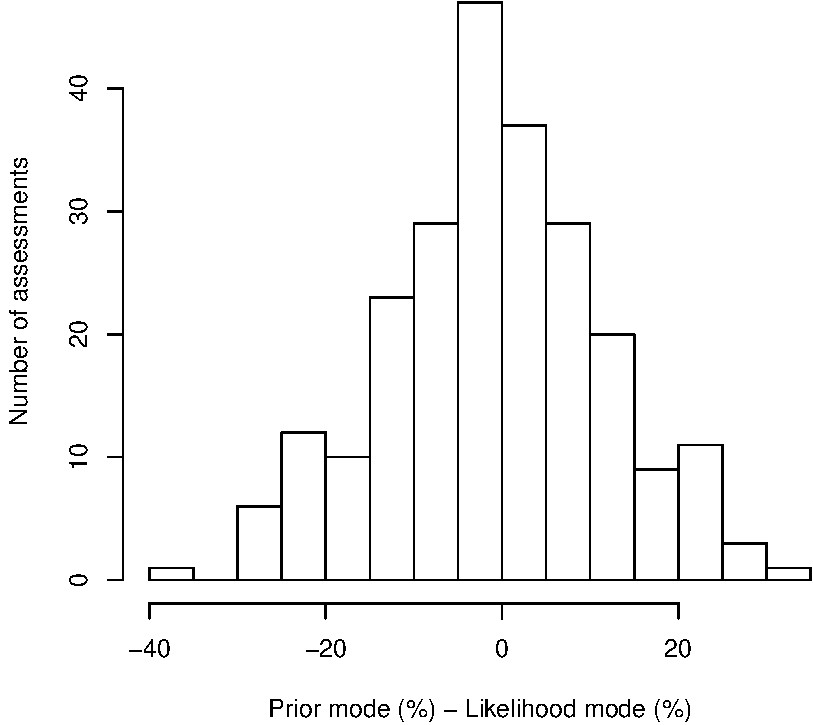
\includegraphics{squeacAttack_files/figure-latex/likehist-1} 

}

\caption{Prior-Likelihood Relationship}\label{fig:likehist}
\end{figure}

\newpage

\hypertarget{scatterplot}{%
\section{Scatterplot}\label{scatterplot}}

\begin{Shaded}
\begin{Highlighting}[]
\KeywordTok{plot}\NormalTok{(results}\OperatorTok{$}\NormalTok{priorMode }\OperatorTok{*}\StringTok{ }\DecValTok{100}\NormalTok{, }
\NormalTok{     results}\OperatorTok{$}\NormalTok{likeMode }\OperatorTok{*}\StringTok{ }\DecValTok{100}\NormalTok{, }
     \DataTypeTok{xlim =} \KeywordTok{c}\NormalTok{(}\DecValTok{0}\NormalTok{, }\DecValTok{100}\NormalTok{), }\DataTypeTok{ylim =} \KeywordTok{c}\NormalTok{(}\DecValTok{0}\NormalTok{, }\DecValTok{100}\NormalTok{), }
     \DataTypeTok{xlab =} \StringTok{"Prior mode (%)"}\NormalTok{, }
     \DataTypeTok{ylab =} \StringTok{"Likelihood mode (%)"}\NormalTok{, }
     \DataTypeTok{pch =} \KeywordTok{ifelse}\NormalTok{(results}\OperatorTok{$}\NormalTok{PLC, }\DecValTok{19}\NormalTok{, }\DecValTok{1}\NormalTok{), }
     \DataTypeTok{frame.plot =} \OtherTok{FALSE}\NormalTok{)}
\KeywordTok{abline}\NormalTok{(}\DataTypeTok{a =} \DecValTok{0}\NormalTok{, }\DataTypeTok{b =} \DecValTok{1}\NormalTok{, }\DataTypeTok{lty =} \DecValTok{2}\NormalTok{)}
\KeywordTok{text}\NormalTok{(}\DecValTok{100}\NormalTok{, }\DecValTok{15}\NormalTok{, }\StringTok{"Prior mode > Likelihood mode"}\NormalTok{, }\DataTypeTok{pos =} \DecValTok{2}\NormalTok{, }\DataTypeTok{cex =} \FloatTok{0.8}\NormalTok{)}
\KeywordTok{text}\NormalTok{(  }\DecValTok{0}\NormalTok{, }\DecValTok{85}\NormalTok{, }\StringTok{"Prior mode < Likelihood mode"}\NormalTok{, }\DataTypeTok{pos =} \DecValTok{4}\NormalTok{, }\DataTypeTok{cex =} \FloatTok{0.8}\NormalTok{)}
\KeywordTok{lines}\NormalTok{(}\KeywordTok{lowess}\NormalTok{(results}\OperatorTok{$}\NormalTok{priorMode }\OperatorTok{*}\StringTok{ }\DecValTok{100}\NormalTok{, results}\OperatorTok{$}\NormalTok{likeMode }\OperatorTok{*}\StringTok{ }\DecValTok{100}\NormalTok{, }\DataTypeTok{f =} \DecValTok{2}\OperatorTok{/}\DecValTok{3}\NormalTok{))}
\end{Highlighting}
\end{Shaded}

\begin{figure}[H]

{\centering 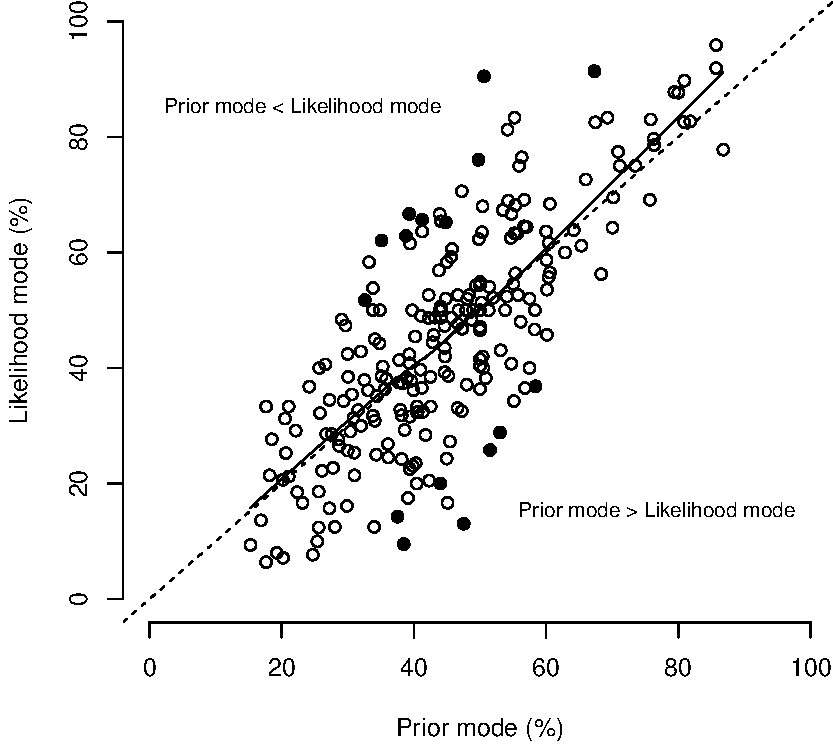
\includegraphics{squeacAttack_files/figure-latex/likescatter-1} 

}

\caption{Prior-Likelihood Relationship}\label{fig:likescatter}
\end{figure}

\begin{Shaded}
\begin{Highlighting}[]
\KeywordTok{cor}\NormalTok{(results}\OperatorTok{$}\NormalTok{priorMode, results}\OperatorTok{$}\NormalTok{likeMode)}
\end{Highlighting}
\end{Shaded}

\begin{verbatim}
## [1] 0.772687
\end{verbatim}

\newpage

\hypertarget{how-precise-is-the-likelihood-estimate-alone}{%
\section{How precise is the likelihood estimate
alone}\label{how-precise-is-the-likelihood-estimate-alone}}

For this, we assume total population of 100,000 with 17\% aged 6-59
months and prevalence of SAM of 2\%.

\begin{Shaded}
\begin{Highlighting}[]
\CommentTok{# Subset to results with PLC == TRUE}
\NormalTok{rejected <-}\StringTok{ }\NormalTok{results[results}\OperatorTok{$}\NormalTok{PLC, ]}
\CommentTok{# calculate number of SAM}
\NormalTok{pop <-}\StringTok{ }\DecValTok{100000} \OperatorTok{*}\StringTok{ }\FloatTok{0.17} \OperatorTok{*}\StringTok{ }\FloatTok{0.02} 
\CommentTok{# calculate finite population correction factor}
\NormalTok{rejected}\OperatorTok{$}\NormalTok{FPC <-}\StringTok{ }\KeywordTok{sqrt}\NormalTok{((pop }\OperatorTok{-}\StringTok{ }\NormalTok{rejected}\OperatorTok{$}\NormalTok{likeD) }\OperatorTok{/}\StringTok{ }\NormalTok{(pop }\OperatorTok{-}\StringTok{ }\DecValTok{1}\NormalTok{))}
\end{Highlighting}
\end{Shaded}

\hypertarget{relative-precision}{%
\subsection{Relative precision}\label{relative-precision}}

\begin{Shaded}
\begin{Highlighting}[]
\CommentTok{# Relative precision of surveys with PLC}
\NormalTok{rejected}\OperatorTok{$}\NormalTok{likeRP <-}\StringTok{ }\NormalTok{(}\KeywordTok{qnorm}\NormalTok{(}\FloatTok{0.975}\NormalTok{) }\OperatorTok{*}\StringTok{ }
\StringTok{                      }\KeywordTok{sqrt}\NormalTok{((rejected}\OperatorTok{$}\NormalTok{likeMode }\OperatorTok{*}\StringTok{ }
\StringTok{                              }\NormalTok{(}\DecValTok{1} \OperatorTok{-}\StringTok{ }\NormalTok{rejected}\OperatorTok{$}\NormalTok{likeMode)) }\OperatorTok{/}\StringTok{ }\NormalTok{rejected}\OperatorTok{$}\NormalTok{likeD) }\OperatorTok{*}\StringTok{ }
\StringTok{                    }\NormalTok{rejected}\OperatorTok{$}\NormalTok{FPC) }\OperatorTok{/}\StringTok{ }\NormalTok{rejected}\OperatorTok{$}\NormalTok{likeMode}

\CommentTok{# Relative precision of an EPI coverage survey with p = likelihood mode, }
\CommentTok{# n = 120, and DEFF = 2.0?}
\NormalTok{rejected}\OperatorTok{$}\NormalTok{epiRP <-}\StringTok{ }\NormalTok{(}\FloatTok{2.0} \OperatorTok{*}\StringTok{ }\KeywordTok{qnorm}\NormalTok{(}\FloatTok{0.975}\NormalTok{) }\OperatorTok{*}\StringTok{ }
\StringTok{                     }\KeywordTok{sqrt}\NormalTok{((rejected}\OperatorTok{$}\NormalTok{likeMode }\OperatorTok{*}\StringTok{ }
\StringTok{                             }\NormalTok{(}\DecValTok{1} \OperatorTok{-}\StringTok{ }\NormalTok{rejected}\OperatorTok{$}\NormalTok{likeMode)) }\OperatorTok{/}\StringTok{ }\DecValTok{210}\NormalTok{)) }\OperatorTok{/}\StringTok{ }\NormalTok{rejected}\OperatorTok{$}\NormalTok{likeMode}

\CommentTok{# How many have relative precision of better than or equal to the }
\CommentTok{# assumed EPI survey?}

\KeywordTok{table}\NormalTok{(rejected}\OperatorTok{$}\NormalTok{likeRP }\OperatorTok{<=}\StringTok{ }\NormalTok{rejected}\OperatorTok{$}\NormalTok{epiRP)}
\end{Highlighting}
\end{Shaded}

\begin{verbatim}
## 
## FALSE  TRUE 
##     6    10
\end{verbatim}

\begin{Shaded}
\begin{Highlighting}[]
\KeywordTok{prop.table}\NormalTok{(}\KeywordTok{table}\NormalTok{(rejected}\OperatorTok{$}\NormalTok{likeRP }\OperatorTok{<=}\StringTok{ }\NormalTok{rejected}\OperatorTok{$}\NormalTok{epiRP))}
\end{Highlighting}
\end{Shaded}

\begin{verbatim}
## 
## FALSE  TRUE 
## 0.375 0.625
\end{verbatim}

\newpage

\begin{Shaded}
\begin{Highlighting}[]
\CommentTok{# Proportion of SQUEAC assessments that fail by ...}
\CommentTok{#}
\CommentTok{#    prior likelihood conflict == TRUE AND precision worse than the }
\CommentTok{#    assumed EPI survey}
\CommentTok{#}
\NormalTok{failN <-}\StringTok{ }\KeywordTok{sum}\NormalTok{(}\KeywordTok{ifelse}\NormalTok{(rejected}\OperatorTok{$}\NormalTok{likeRP }\OperatorTok{>}\StringTok{ }\NormalTok{rejected}\OperatorTok{$}\NormalTok{epiRP, }\DecValTok{1}\NormalTok{, }\DecValTok{0}\NormalTok{))}
\NormalTok{failP <-}\StringTok{ }\KeywordTok{round}\NormalTok{(}\KeywordTok{sum}\NormalTok{(}\KeywordTok{ifelse}\NormalTok{(rejected}\OperatorTok{$}\NormalTok{likeRP }\OperatorTok{>}\StringTok{ }\NormalTok{rejected}\OperatorTok{$}\NormalTok{epiRP, }\DecValTok{1}\NormalTok{, }\DecValTok{0}\NormalTok{)) }\OperatorTok{/}\StringTok{ }
\StringTok{                 }\KeywordTok{nrow}\NormalTok{(results) }\OperatorTok{*}\StringTok{ }\DecValTok{100}\NormalTok{, }\DecValTok{2}\NormalTok{) }

\KeywordTok{print}\NormalTok{(failN)}
\end{Highlighting}
\end{Shaded}

\begin{verbatim}
## [1] 6
\end{verbatim}

\begin{Shaded}
\begin{Highlighting}[]
\KeywordTok{print}\NormalTok{(failP)}
\end{Highlighting}
\end{Shaded}

\begin{verbatim}
## [1] 2.52
\end{verbatim}

\newpage

\renewcommand\refname{References}
\bibliography{bibliography.bib}


\end{document}
